\setAuthor{Erkki Tempel}
\setRound{lahtine}
\setYear{2018}
\setNumber{G 1}
\setDifficulty{1}
\setTopic{Geomeetriline optika}

\prob{Kärbes}
Kärbes asub kumerläätse fokaaltasandil, läätse optilisest peateljest kaugusel $a = \SI{1}{m}$ ning hakkab lendama läätse kahekordse fookuskauguse suunas kiirusega $v = \SI{0,5}{m/s}$. Läätse fookuskaugus $f = \SI{1}{m}$. Millise kiirusega $u$ liigub kärbse kujutis sel hetkel, kui kärbse ja tema kujutise vaheline kaugus on minimaalne?
\begin{center}
	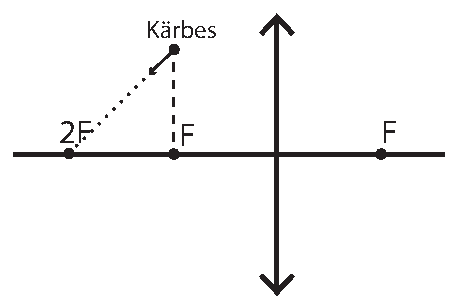
\includegraphics[width = 0.5\linewidth]{2018-lahg-01-yl.pdf}
\end{center}\hint

\solu
Minimaalne kaugus on siis, kui kärbes läbib optilist peatelge. Kärbes ja tema kujutis on sel hetkel läätsest kahekordse fookuskauguse kaugusel. Kuna nii kärbes kui ka tema kujutis on läätsest sama kaugel, on kujutise suurendus $1$, mistõttu kujutise liikumiskiirus on sama, mis kärbse liikumiskiirus, ehk $u = v = \SI{0,5}{m/s}$.
\probend